%%%%%%%%%%%%%%%%%%%%%%% file template.tex %%%%%%%%%%%%%%%%%%%%%%%%%
%
% This is a general template file for the LaTeX package SVJour3
% for Springer journals.          Springer Heidelberg 2010/09/16
%
% Copy it to a new file with a new name and use it as the basis
% for your article. Delete % signs as needed.
%
% This template includes a few options for different layouts and
% content for various journals. Please consult a previous issue of
% your journal as needed.
%
%%%%%%%%%%%%%%%%%%%%%%%%%%%%%%%%%%%%%%%%%%%%%%%%%%%%%%%%%%%%%%%%%%%
%
% First comes an example EPS file -- just ignore it and
% proceed on the \documentclass line
% your LaTeX will extract the file if required
\begin{filecontents*}{example.eps}
%!PS-Adobe-3.0 EPSF-3.0
%%BoundingBox: 19 19 221 221
%%CreationDate: Mon Sep 29 1997
%%Creator: programmed by hand (JK)
%%EndComments
gsave
newpath
  20 20 moveto
  20 220 lineto
  220 220 lineto
  220 20 lineto
closepath
2 setlinewidth
gsave
  .4 setgray fill
grestore
stroke
grestore
\end{filecontents*}
%
\RequirePackage{fix-cm}
%
%\documentclass{svjour3}                     % onecolumn (standard format)
%\documentclass[smallcondensed]{svjour3}     % onecolumn (ditto)
\documentclass[smallextended]{svjour3}       % onecolumn (second format)
%\documentclass[twocolumn]{svjour3}          % twocolumn
%
\smartqed  % flush right qed marks, e.g. at end of proof
%
\usepackage{cite}

\newcommand{\pluseq}{\;\mathrel{{+}{=}}\;}
\newcommand{\asteq}{\mathrel{*}=}
\usepackage{inconsolata}
\usepackage{graphicx}
\usepackage{url}
\usepackage{colortbl}
\usepackage[usenames,dvipsnames]{xcolor}
\usepackage{tikz}
\definecolor{alizarin}{rgb}{0.82, 0.1, 0.26}

\newcommand*\circled[1]{\tikz[baseline=(char.base)]{
            \node[minimum width=1pt, shape=circle,fill=black,inner sep=.1pt] (char) {{\scriptsize \textcolor{white}{#1}}};}}

\newcommand{\one}{\circled{1}}
\newcommand{\two}{\circled{2}}
\newcommand{\three}{\circled{3}} 
\newcommand{\four}{\circled{4}}
\newcommand{\five}{\circled{5}}
\newcommand{\six}{\circled{6}}
\newcommand{\seven}{\circled{7}}
\newcommand{\eight}{\circled{8}}
\newcommand{\nine}{\circled{9}}
\newcommand{\ten}{\circled{10}}
\newcommand{\eleven}{\circled{11}}
\newcommand{\twelve}{\circled{12}}
\newcommand{\thirteen}{\circled{13}}
\newcommand{\fourteen}{\circled{14}}
\newcommand{\fifteen}{\circled{15}}
\newcommand{\sixteen}{\circled{16}}
\newcommand{\seventeen}{\circled{17}}
\newcommand{\eighteen}{\circled{18}}
\newcommand{\nineteen}{\circled{19}}
\newcommand{\twenty}{\circled{20}} 

\definecolor{CustomDarkRed}{RGB}{175, 0, 0} 
\newcommand{\RED}[1]{{\color{CustomDarkRed}\texttt{\textbf{#1}}}}

\makeatletter
\newcommand\notsotiny{\@setfontsize\notsotiny\@vipt\@viipt}
\makeatother

\definecolor{LightGray}{gray}{0.978}
  
\usepackage{minted}
\setminted{%
baselinestretch=.9,%
%frame=lines,% 
%firstnumber=last,%
%xleftmargin=20pt,% 
%numbers=right,%
%framesep=3mm,% 
   % autogobble,%
escapeinside=||,%
%numbersep=4pt,%
bgcolor=LightGray,
%bgcolor=LightGray,%
fontsize=\scriptsize,%
linenos=off
}
\usemintedstyle{trac}

 
%
% \usepackage{mathptmx}      % use Times fonts if available on your TeX system
%
% insert here the call for the packages your document requires
%\usepackage{latexsym}
% etc.
%
% please place your own definitions here and don't use \def but
% \newcommand{}{}
%
% Insert the name of "your journal" with
% \journalname{myjournal}
%

% \usepackage[T1]{fontenc}
% \usepackage{libertine}%% Only as example for the romans/sans fonts
% \usepackage[scaled=0.85]{beramono}
\begin{document}
\newcommand{\eg}{{\sffamily  EG}}
 

\title{Optimizing  optimization
via predictive models}
%\thanks{Grants or other notes
%about the article that should go on the front page should be
%placed here. General acknowledgments should be placed at the end of the article.}
% }
 

%\titlerunning{Short form of title}        % if too long for running head

\author{Tim Menzies
}

%\authorrunning{Short form of author list} % if too long for running head

\institute{Tim Menzies \at
              Computer Science, NC State \\ 
              \email{timm@ieee.org}           %  \\
%             \emph{Present address:} of F. Author  %  if needed 
}

\date{Received: date / Accepted: date}
% The correct dates will be entered by the editor


\maketitle

\begin{abstract}
In this special issue on predictive modeling, we study  models for software analytics  that    predict the effectiveness of an optimizer.  In turns out, that for many SE domain,
it takes very little data to train a predictive  model that can guess if an optimizer will like/dislike the next example.  Using these models, software analytics can  stop early (since this predictive model can be used for   the subsequent reasoning).


To test this approach, we explore
27  challenge problems (ranging from
from high-level decisions about software processes to low-level decisions abut how to
configure video encoding software). When these problems have
been previously explored by software engineering researchers, they required hundreds to thousands to millions
of labelled examples. 
Here, we achieve significant improvements using just a handful of examples (sometimes, as few as 12 labels).  


Other SE researchers have explored    model building
using   limited labelling via  unsupervised or semi-supervised learning, or active learning, or zero/few-shot learning.
But to the best of our knowledge, 
this paper's success with only a handful of examples
(and no large language model) is unprecedented.  

We call this approach LITE since it is  inherently different to HEAVY methods that (e.g.) need a large language
model for some generative task
(such as code translation). As
shown in this paper, not all SE tasks are HEAVY. Hence it is
prudent to research both LITE and HEAVY methods

This    LITE approach is   recommended for   human-in-the-loop process where humans have to  assess   the  examples (e.g. humans are generating the labels; or humans are assessing the examples used in building a model).

In accordance with the principles of open science, we offer the reproduction package of \url{XXX}
to allow others to repeat/refute/improve these results.


 

  

% Over the years, there have been many reports that very simple models can perform exceptionally well. Yet, where are the researchers asking ``say, does
% that mean that we could make software analytics simpler and more comprehensible?''
%  This is an important question, since humans often have difficulty accurately assessing complex models (leading to unreliable and sometimes dangerous results). 
 
%  Prior PROMISE results have shown that data mining can effectively summarizing large models/ data sets into simpler and smaller ones.  Using that experience, this paper presents and tests LAB (the Lightweight Adaptive Balancer).
%  LAB takes a tree of Parzen estimator approach to incremental model construction;
%  i.e. build a model from a handful of examples (divided into ``best'' and ``rest'')
%  then use than model to select what example to label next. 

%   In case studies with 30 different  multi-objective tasks  
%     our LAB tool
% (the Lightweight Adaptive Balancer)  could use Bayesian sequential
% model optimization to find large changes that improved
%   default behavior of these systems, after just labelling two dozen examples.
%   This result held even when that case study contained tens of thousands of unlabelled examples. 
%   This result is unique since when these case studies were explored previously, SE researchers needed thousands to millions of labelled examples.  

%   We hence make a ``non-big-data'' conclusion that  
%   tools like LAB are useful when humans have to quickly learn what they can about
%   some model, without having to first label 100s of examples (or more).

  
\keywords{Predictive Modeling \and
Search-based SE \and 
Software Engineering
% \PACS{PACS code1 \and PACS code2 \and more} 
}
\end{abstract}


%  LAB  would explore (say) 10,000 unlabelled items as follows: \newline
% (a)~use N=4 evalaution to label four   items ; \newline 
% (b)~divide labelled items into ``best'' and ``rest'' using a multi-goal criteria;\newline  (c)~build  a  classifier 
% to find, for unlabelled item, B=like(``best''), R=like(``rest'');\newline 
% (d)~sort, in ascending order, the remaining    9996 items  by -B/R; \newline  
% (e)~label the  top item (so N=N+1), and
% discard the last 20\%   unlabelled items;\newline  (f)~update best and rest with this new item; \newline  (g)~if N$<$25,   loop back  to (b). Else terminate, returning the top item in          ``best''.




\newpage\section{Introduction}\label{intro} 
This paper  explores  models for software analytics that    predict the effectiveness of an optimizer.  We will show that for many SE domain,
it takes very little data to train a predictive  model that can guess if an optimizer will like/dislike the next example.  
Using these
models, software analytics can stop early (since this predictive model can be
used for the subsequent reasoning). We call this approach  ``LITE'':
\begin{quote}
    {\bf LITE } = Low Input Tuning Enhancement: {\em
 improve a software system’s behavior
without having to spend much effort labelling local data. }
\end{quote}
%  A similar approach to LITE can be found in    search-based SE~\cite{sarro2023search} where it is assumed that improving
% system behavior is a multi-objective problem that must  trade-off between competing concerns. But unlike, standard SBSE, 
LITE addresses the {\em labelling problem}. One way to study some system ``$f$''   
 is to explore examples  {\eg}s$\;=(X,Y)$ where $X=f(Y)$.
 Here,   $X$ are the independent variables
and $Y$ are one or more numeric dependent goal variables.  
{\eg}s are usually created without $Y$ values and 
{\em labelling} is the process of reading   $X$   in order to compute   $Y$.
LITE assumes
we can only label dozens, not thousands  of {\eg}s. As such,
LITE is very amenable to human-in-the-loop reasoning where 
humans have to assess the {\eg}s (e.g. humans are generating the labels; or
humans are assessing the {\eg}s used in building a model) 


An alternative to LITE are HEAVY methods that assume ``the more {\eg}s the better''-- an approach   endorsed by many SE researchers; e.g.~\cite{mcintosh2017fix,rahman2013sample,amasaki2020cross}. 
Some SE tasks are inherently HEAVY, such as the   creating   a large language model for use on  generative tasks such as code translation~\cite{10.1145/3551349.3559555}. That said, as shown in this paper, not all SE tasks need a HEAVY approach. Hence it is prudent to research both LITE and HEAVY methods.

To kick start the LITE research agenda, this paper, in  \S\ref{why},
    makes the business case for studying  LITE-style reasoning.
    Next, in 
  \S\ref{label} we detail the labelling problem, and why we should
    avoid over-labelling.
    This is followed, in  \S\ref{how} by a discussion on why the problems addressed by  LITE  are not solved
    by current research into interactive SBSE, active learning, unsupervised and semi-supervised learning, and zero/few-shot learning.
    After that,  \S\ref{lite}  describes \verb+lite.py+, a tiny
    implementation of a multi-objective TPE (tree-structured Parzen estimator) that   implements incremental model construction;   i.e. build a model from a handful of labelled {\eg}s (divided into ``best'' and ``rest'')
    then use than model to select what to label next.
  
    \S\ref{data} describes  case studies from the SE optimization literature. Prior work in SE needed  thousands to millions of labels for these   studies.
    But as we shall see in \S\ref{out},  \verb+lite.py+'s       significantly improves the default
    behavior seen in those problems, sometimes after  just half a dozen labels.
    To the best of
our knowledge, this is the fewest   labels ever used for these tasks in SE.

  Finally, to encourage further work,   \S\ref{next}   offer twenty challenge problems that could be readily explored using \verb+lite.py+ and the 27 case studies.
Our hope is that numerous researchers repeat our experiments and discover
methods that are superior to the one proposed here. Paradoxically, this means
this paper will be a success if it is quickly superseded.

\section{The Business Case for LITE}\label{why}
 % In essence, LITE asks what does it take to change a system 
 % from (a)~its default behaviour  to (b)~some preferred option. This section
 % argues that humans will increasingly need support for this kind of reasoning.



Enabling humans to explore  the important potential behaviors of a software model is an open and important  issue. 
For example,
the more we use AI in SE, the more code will be auto-generated.
The more we auto-generate code,    software engineers will   spend less
time  writing new code and time
reviewing code, written by someone or something else (the internals of which they may not understand).
The less we  
understand code, 
the more we will use components  black-boxes  
  where once a system is assembled, its control settings
are tuned.  
In this scenario, it becomes very  important to reduce
the human effort and CPU effort required for that tuning.


We predict that enhancing our ability to reviewing models will become increasingly important in SE.
In  
``Flaws of policies of requiring human oversight''~\cite{green2022flaws},
Ben Green notes that many recent policies      require humans-in-the-loop to review or   audit   decisions from software models. 
E.g. the  manual of the
(in)famous  COMPAS model notes the algorithm can make mistakes and advises that 
``staff should be encouraged to use their professional judgment and override the computed risk as appropriate''~\cite{northe15}. 

Cognitive theory~\cite{simon1956rational} tells us that
  humans  use heuristic ``cues'' that lead them to the most important parts 
of a model before moving on to their next
task. But when humans review models, they can miss important details. Such cues are essential if humans are to tackle
their busy workloads. That said,  using cues can introduce errors:
   {\em 
   ...people (including experts) are susceptible to ``automation bias'' (involving)  omission errors—failing to take action because the automated system did not provide an alert—and commission error}~\cite{green2022flaws}.
 This means  that   oversight policies   can lead to the reverse of their desired effect  by {\em ``legitimizing the use of   faulty and controversial algorithms without addressing (their fundamental issues''}~\cite{green2022flaws}. 





%.  

%Cognitive theory~\cite{simon1956rational} tells us that humans  use heuristic ``cues'' that lets them find    (hopefully)  most important parts of a modelbefore rushing off to their next task.


 
  Sadly,
there are too many examples of such errors:
\begin{itemize}

\item
Widely-used face recognition software   predicting    gender \& age, has a much
higher error rate for dark-skinned women compared to light-skinned men~\cite{Skin_Bias}.
\item  Amazon's  delivery  software    became   biased against black neighborhoods \cite{Amazon_Bias}. 
\item
  Google Translate  has gender bias. ``She is an engineer, He is a nurse''   translates    Turkish then
     English as ``He is an engineer, She is a nurse'' \cite{Caliskan183}.
  \item The COMPAS model guesses that  black defendants as future criminals   twice as much   as whites~\cite{Machine_Bias}.
  It took years to find and fix this bug
  (and that difference is definitely  a bug since it can be fixed~\cite{fse21} while  maintaining the same levels of recall on actual recidivism).
  \item For  other examples, see~\cite{rudin2019explaining,noble2018algorithms,gebru21}.
\end{itemize}
% 
%That difference is a bug (and we know that is a  bug since it can be fixed-- see PI Menzies' FSE'21 paper~\cite{fse21} that weights training examples to reduce COMPAS's false alarm delta, while  maintaining the same levels of recall on actual recidivism).
% \begin{table}[!b]
% \begin{tabular}{|p{.98\linewidth}|}\hline
% \rowcolor{blue!10}   COMPAS guesses that  black defendants as future criminals   twice as much   as whites~\cite{Machine_Bias}.
% \\
% Widely-used face recognition software   predicting    gender \& age, has a much
% higher error rate for dark-skinned women compared to light-skinned men~\cite{Skin_Bias}.
% \\
% \rowcolor{blue!10} Amazon's   software for same-day delivery    became   biased against black neighborhoods \cite{Amazon_Bias}. 
% \\
%   Google Translate  has gender bias. ``She is an engineer, He is a nurse''   translated to  Turkish then
%   back to  English gives ``He is an engineer, She is a nurse'' \cite{Caliskan183}.\\\hline
% \end{tabular}
% \caption{ Example biases seen in   software decisions. For  other examples, see~\cite{rudin2019explaining,noble2018algorithms,gebru21}.
% }\label{tbl:sigh}
% \end{table}
To forge an effective partnership, humans and artificial intelligence (AI) need to understand each other's strengths and limitations. Software can explore a very large space,
on pre-determined criteria. But humans can offer important and useful insight, but only over
a small number of instances. We are interested in tools like 
LITE
since  they do not make excessive demands of humans reviewing software systems.



\section{  Problems with Labelling}\label{label}


In SE, the usual case is that  is very cheap to find $X$ values but far  more expensive to find   $Y$. For example, by mining Github, it is possible to discover all the $X$ distributions of code size, number of dependencies per function, etc. But it can be far more complicated to find the  associated $Y$ values like ``how much this could be sold on the market?'' or ``what is the time required
to build this kind of software?''. For example, the SZZ algorithm reports what code is associated with a  bug fixing commit. Any number of papers report the complexity of making that determination~\cite{herbold2022problems,ROSA2023111729}.

Many labels are naive or faulty. 
Defect prediction researchers~\cite{catolino2017just, hindle2008large, kamei2012large, kim2008classifying, mockus2000identifying} often  label a commit as "bug-fixing" when the commit text uses words like "bug, fix, wrong, error, fail, problem, patch ." Vasilescu et al.~\cite{vasilescu2018personnel, vasilescu2015quality} warns that this can be somewhat ad-hoc, particularly if researchers just peek at a few results, then tinker with regular expressions to combine a few keywords.
 Also, when Yu et al.~\cite{9226105} explored labels from prior work exploring technical debt, they found that more than 90\% of labels marked as "false positive" was true. In the SE literature, there are similar reports where data labels error have corrupted the majority of the {\eg}s for security bug labeling~\cite{ 9371393}; for labeling false alarms in static code analysis~\cite{10.1145/3510003.3510214}; or for software code quality~\cite{Shepperd13}.
    
Not only can labelling be error prone, it can  also be very expensive. 
For example, Tu. et al.~\cite{tu2020better}   studied  714 software projects, including 476K commit files. After an extensive analysis, they  proposed a cost model for labeling their {\eg}s. Assuming two people checking per commit, that data would need three years of effort to label their {\eg}s. 

Since labelling is error-prone, expensive and/or time-consuming, we explore methods that use     as few labels as possible.
One reason
to use minimal labels is that this simplifies the review process described in the last section. Specifically, is is simpler to audit a system when that review means   reflecting over the handful of {\eg}s used used to build the model.  


Before going on, we   offer one piece of nomenclature about labels. For an {\eg} with goal labels $Y$, each  goal
has a range \mbox{ {\em lo .. hi}} and so
can be normalized 0..1. Each goal 
has a  {\em heaven}  of  0,1 if 
 that goal is to be  minimize or maximized  (respectively). We say an example has a distance to heaven ({\em d2h}) equal to the Euclidean distance of the goal values to a mythical best value. For example, if we want to minimize
\textit{ bugs} and \textit{features}, and these have the  range 0 to 100, then for an example with 30 \textit{bugs} and 80 \textit{features}:
 

{\small \begin{equation}\label{d2h}
{\scriptsize  
\mathit{d2h}((X,Y))  = \mathit{dist}(\mathit{heaven}, \mathit{norm}(Y)) =  \sqrt{ (0-.3)^2 +  (1-.8)^2}/\sqrt{2} = 0.26
}
\end{equation}}
Note that {\em smaller} values of \textit{d2h} are \textit{better}.
Also we dividing the distance by the $\sqrt{|\mathit{goals}|}$, to ensure    \textit{d2h} has a range zero to one. 



% Other cost models are just as pessimistic:
% \begin{itemize}
%     \item  Valerdi~\cite{valerdi2010heuristics} documentes  the effort associated with getting a panel of experts to agree on the labels of 60 software project effort estimation examples, where each example has 20 attributes. That study required 3*three hour sessions, spread out over one working week. 
%     \item Researchers in the field
%     of repertory grids conduct structured interviews where humans justify attributes and attribute settings for    random subsets of 3 examples, drawn from a larger set. 
%     \begin{itemize}
%     \item
%     Kington~\cite{kington2009defining} reports that it takes humans hour to reflect over  16 examples with 16 attributes.
%     \item
%     Easterby-Smith~\cite{EASTERBYSMITH19803} advises ``keep the grid small. A grid containing ten elements and ten constructs may take two hours to complete. Larger grids may take substantially more time''.
%    \end{itemize}
%    \eind{itemize}
    
     
% \end{itemize}
\section{How Many Labels are Enough?}
The previous section warned  that it is unwise (and expensive) to expect or rely on large libraries of labelled data. This section asks  ``at what rate can we expect to collect high-quality labels?''.
Here we explore 
 some knowledge acquisition exercise where SMEs (human subject-matter experts) have to carefully justify all their decisions (perhaps even to a panel of other experts).  
 
Acquisition of high-quality labels from humans experts can  be remarkably slow. Valerdi~\cite{valerdi2010heuristics} documents  the effort associated with getting a panel of experts to agree on the labels of 60 software project effort estimation examples, where each example has 20 attributes. That study required 3*three hour sessions, spread out over one working week. 

Other research offers similar numbers to Valerdi. Researchers in the field
    of {\em repertory grids} conduct structured interviews where humans justify attributes and attribute settings for    random subsets of 3 examples, drawn from a larger set. 
    \begin{itemize}
        \item
    Easterby-Smith~\cite{EASTERBYSMITH19803} advises ``keep the grid small. A grid containing ten elements and ten constructs may take two hours to complete. Larger grids may take substantially more time''.
    \item
Kington~\cite{kington2009defining} agrees, saying  that it takes humans an hour to reflect over  16 examples with 16 attributes.
   \end{itemize}
Anyone who has worked with real-world SMEs know that experts are experts precisely because their expertise is valuable to the organization. 
This means that, by definition,
the SMEs needed for high quality labelling may often   called away to other tasks. In our experience:
\begin{itemize}
\item
  Initially, this kind of senior-level expertise can only be accessed for a few hours per month.
  In these initial sessions, SMEs might be interested in your techniques, but will soon abondon you if there is nothing to show for their valuable time.
  \item More access to more labelled data can be achieved--  but only  if substantive results are achieved with the few labels collected from the initial sessions.
  \end{itemize}
Accordingly, the goal of this paper is to understand what happens if we can only access 80,40,20 or even as few as 10  labels.




\section{Methods for Labelling Less}\label{how} 
Other SE researchers have explored    model building
using a few labelled {\eg}s.  But as we shall see in this section,
(with some caveats) those method are rarely applied on as little as 80,40,20 or 10 labels.

There are two kinds of algorithms that make decisions about software without   new labels from the test domain.
 \underline{\bf  Zero-shot learners} use  the  background knowledge of a large language model to make decisions without needing new labels~\cite{alhoshan2022zero}.
 Zero-shot learners  works in domains where there exists an
  appropriate language language model (which is {\em not}
  the situation for our case studies).
Apart from zero-shot learners,
 traditional  \underline{\bf unsupervised learners} use a domain heuristic to classify examples by 
 peeking at the independent variables:
 E.g. Nam et al. successfully predict for defective modules by looking for classes that are unusually large~\cite{nam2015clami}.  For our case studies, we know of no such domain heuristics.

 Another technique for labelling less is to recognize  some system condition
 under which an {\eg}
can be unequivocally labelled as ``fail''; e.g. (a)~if a test generates a core dump or (b)~some metamorphic predicate~\cite{chen2018metamorphic} argues that, say, ``small changes to inputs should not cause large changes to 
output'':
\begin{itemize} 
\item The value of this approach is that such a domain-general labelling
oracle  might be relevant to other applications.
\item On the flip side, the more general the test oracle, the less it connects
to the specific goals of the local users.
 For example, in the case studies shown below, we test for user-supplied 
 local goals such as ``if we implement this requirement next, then some other team will not stand idle waiting for some other function we were meant to implement''.
 \end{itemize} 
 Another class of algorithms use less labels by, say,    labelling just a few {\eg}s,  then propagate those values to other near-by {\eg}s.
Such  \underline{\bf semi-supervised} learners have successfully reasoned over 10,000s   records, after labelling just 1 to 2.5\% percent of the {\eg}s~\cite{10109333,majumder2024less}.
While a useful approach, these method   still needs 
100s to 1000s  of labels. 

Human-in-the-loop   \underline{\bf  active learners}  
minimize human labelling effort by updating their models
each time a human offers an opinion on an {\eg}.
Still, even with these tools, the labelling effort can be excessive.
Yu et al.'s active learners need 20\% of the data
labelled, which for (e.g.) 28,750 files in Firefox means labelling 5,750 {\eg}s~\cite{yu2019fast2}. Similar values of 10 to 20\% labelling
have been reported by other active learning researchers in SE:
see   Wu et.al~\cite{WU2021106530}.

Researchers in  \underline{\bf  interactive-search-based SE} explore human-in-the-loop optimization where humans serve as the oracle that judges  if one {\eg} is better than another.
The problem
with iSBSE is that when humans are asked too many questions,
they start making mistakes due to  {\em cognitive fatigue}~\cite{shackelford2007implementation}.
One solution to this problem is to learn a {\em surrogate model} from a small sample of {\eg}s, then querying the surrogate for labels~\cite{araujo2017architecture}.  But even with technologies like surrogates, our reading of the iSBSE
research~\cite{lin2016interactive,amal2014use,araujo2017architecture} is that community still assumes they can  label hundreds of examples, or more.

In the SE literature, one area close to this paper
is
\underline{\bf few-shot learning}.
This is a technique that uses 
a few dozen  labeled {\eg}s (sometimes as few as ten)   
to convert a general large  language models into some specific tool; e.g. 
 parsing   test  case output~\cite{le2023log} or translating functions into English~\cite{10.1145/3551349.3559555}. But
 like zero-shot learning, few-shot learning
 only works where, in the domain being explored, there exists
 a functioning large-language model. As we shall see, there are many domains in SE where this is not true.

\subsection{Prior Work with ``SWAY''}\label{sway}
In our own prior work, the closest approach we have to LITE are  the   recursive random projections of SWAY~\cite{Chen19}. 
% nd the tabu search of DODGE~\cite{agrawal2019dodge}. 
% DODGE used 30 labels while SWAY's
% binary-chop approach only  labelled 
% around $\log(N)$ of the {\eg}s.  
SWAY was inspired by   algorithms that clustered data using  PCA (principle components analysis~\cite{pearson1901principal}).
The advantage of PCA is that some data sets are better described by synthesized attributes that combine the influences of raw attributes.
But standard PCA can only handle numeric data so SWAY combined the Aha et al.~\cite{aha91} distance metric\footnote{ Aha et al.~\cite{aha91}  suggest that points $(X_1,Y_1), (X_2,Y_2)$ are
separated by $\mathit{dist}(X_1,X_2)= \left(\sum_i \Delta(X_1^{'},X_2^{'})^2\right)^{0.5}$. For discrete values, 
\mbox{$\Delta(a,b)=0\;\mathit{if}\;a==b\;\mathit{else}
\;1$}.
For numeric values,
$\Delta(a,b) = 
\mathit{abs}(\hat{a} - \hat{b})$ where $\hat{a}$ is $a$   normalized to the range 0..1 for min..max.
For missing values, we use values for 
$a,b$ that maximizes the computed distance.
}
with the FASTMAP heuristic\footnote{To 
  recursively bi-cluster data, first pick any {\eg}  at random; 
  then use the Aha metric to find a remote  example, called $A$.
  Next, find the  example $B$ furthest from $A$ and label $A,B$ ``best'' and ``rest'' using   Equation~\ref{d2h}.
If every other {\eg} have a distance $a,b$ to $A,B$, then all those points fall on a line between $A,B$ at $x=(a^2+c^2-b^2)/(2c)$, where  $c=\mathit{dist}(A,B)$.
After splitting on median $x$, then this algorithm recursive on ``best'' half. 
This approach is fast since each level of this recursion only requires $2N$ distance calculations.}~\cite{faloutsos1995fastmap} to recursively bi-cluster {\eg}s using the independent attributes. Formally, SWAY belongs to the family of Nystr\"om algorithms that approximate PCA, by various methods~\cite{platt2005fastmap}.
 
  SWAY  
   implement optimization as a binary chop through a space of {\eg}s
   clustered as per the last paragraph.
 At each level of the recursion, SWAY uses FASTMAP and Aha to find two distant examples $A,B$. It then sorts them into ``best'' and ``rest'' using Equation~\ref{d2h}.  SWAY then recurses on the examples nearest the ``best''.  
 On recursion, when looking for two more distant points, SWAY 
 reuses (without relabelling) the  ``best'' {\eg} from the  parent. This means that SWAY needs two evaluations for the root split (since, there,  there is no parent cluster), then one new labelling for each level of recursion.


 SWAY terminates
when leaf classes contain less than some user-specified point; e.g. $\sqrt{N}$. 
On termination, it returns the last ever ``best'' example found by the algorithm.
For clustering $N=10,000$ examples into bins of size $\sqrt{N}=100$, SWAY requires nine labels. 

%\section{\verb+lite.py+}

 SWAY is a ``greedy search''; i.e.  it
  decisions using purely local information.   Such a search is   susceptible to premature commitments since  it might prune good {\eg}s without
enough reflection.

% In an experiment with a non-greedy approach that revisits some of SWAY's decisions, this paper explores  SWAY2,   which calls SWAY to find one best  big leaf clusters of size 50, 
% once again on those 50 {\eg}s
% to find leaf clusters of size 4
% (which are then all labelled).
% For $N=10000$ {\eg}s,
% SWAY2 needs 16 evaluations to select a single preferred {\eg}.  

An alternative to SWAY's greedy search is the 
  predictive modeling approach of   
\verb+lite.py+.
That algorithm  rebuilds its knowledge every time is sees a new {\eg}, then
searches afresh over the unlabelled data from the next thing to label.,
The experiments of this paper will show that the 
 predictive modeling of \verb+lite.py+   out-performs 
  SWAY's greedy search.

% \subsection{DODGE}

% The  
%    DODGE hyperparameter optimizer~\cite{agrawal2019dodge}. 
%  DODGE was a tabu search that encouraged an optimizer to avoid new {\eg}s   that generated solutions that were too close
% to old solutions.   
% DODGE   only needed 30 {\eg}s
% to configure learners for  for a range of SE tasks. 

% To our shame,  DODGE was never compared to  a purely random selection of 30 {\eg}s until several years after its publication. While we cannot not defend that oversight, we note that ``compare with random'' does not appear in SE's lists of ``best practices'' for this kind of research:
% \begin{itemize}
% \item
% Such comparisons are not mentioned in {\S}9 of the    Arcuri\& Briand text~\cite{10.1145/1985793.1985795}.
% \item
% In the Empirical SE standards docs at 
% \url{https://github.com/acmsigsoft/EmpiricalStandards}, footnote 7 of 
% docs/standards/OptimizationStudies.md suggests that such random comparisons are depreciated.
% \end{itemize}
% In any case, 
% DODGE is not reported in this since the ``compare with 30 random condigurations'' results reported below typically performed as well as DODGE.  




\section{Predictive Modeling with {\tt lite.py}}

XXX need an example here

As stated in the introduction, one of the stated aims of this paper is to encourage much experimentation with a LITE approach to software analytics. Hence it is apropos to note that the source code for \verb+lite.py+ (and, indeed, SWAY)
is very short. 



Oune problem with 
If DODGE is out-perform by ``compare with 30 random {\eg}s'', then why go any further? Why not    recommend that all optimizations of local data just tries 30 random {\eg}s, then stop?

For two reasons, we need to do better than    ``use 30 random''. Firstly, random search  returns  nothing at all except a set of {\eg}s, sorted by some criteria.
This is undesirable.
Ideally, we want an optimization study to return    a generalizable model that can be applied to future {\eg}s:
\begin{itemize} 
\item Without such a generalizable model, then if ever we have to repeat an optimization study, that second study will take as much effort as the first study.
\item But with such a generalizable model, if that second study   reuses the model
learned from the first study, the it may be possible to avoid any further labelling.
\end{itemize}
Secondly, another reason to do better than ``use 30 random'' is that
  30 labels may be too many. This is
particularly true  if those labels are collected from 
SMEs (human subject matter experts).



 


 The more society depends on software, the more likely it becomes that some organizational policy or some legislative requirement will demand that
 that software gets evaluated. 
Green~\cite{green2022flaws}  comments that when faced with large and complex problems,
  cognitive theory~\cite{simon1956rational} tells us that humans use heuristic ``cues'' to lead them to the most important parts
of a model.   Such cues are essential if humans are to reason about large problems.   

That said,  using cues can introduce their own errors:
   {\em 
   ...people (including experts) are susceptible to ``automation bias'' (involving) omission errors - failing to take action because the automated system did not provide an alert - and commission error}~\cite{green2022flaws}.
 This means that oversight can lead to the opposite desired effect by {\em ``legitimizing the use of faulty and controversial (models) without addressing (their fundamental issues'')}~\cite{green2022flaws}. 

By ``faulty and controversial models'', Green refers to
the  long list of examples where detrimental models  were learned via
algorithmic means.
For example,   Cruz et al.~\cite{cruz2021promoting}  lists examples where:
\begin{itemize}
\item Proposals from low-income groups are five times more  likely     to be incorrectly ignored by donation groups;
\item Women can be five times more likely to be incorrectly classified as low-income;
\item African Americans are five times more likely to  languish in prison until trial,
rather given the bail they deserve.  
\end{itemize}
These are just a few of the many reported examples\cite{rudin2019explaining}\footnote{See also 
\url{http://tiny.cc/bad23a}, \url{http://tiny.cc/bad23b}, \url{http://tiny.cc/bad23c}} of algorithmic discrimination.
For another example, the last chapter of Noble~\cite{noble2018algorithms} describes how a successful
hair salon went bankrupt due to internal
choices within the YELP recommendation algorithm.

 
Mathews~\cite{mathews23} argues that it is not surprising that so many She  notes that everyone seeks ways to exploit some advantage for themselves. Hence, we should
expect that the software we build to discriminate against some social groupings;
\begin{quote}

{\em 
    ``People often think of their own hard work or a good decision they made. However, it is often more accurate to look at advantages like the ability to borrow money from family and friends when you are in trouble, deep network connections so that you hear about opportunities or have a human look at your application,  the ability to move on from a mistake that might send someone else to jail, help at home to care for children,  etc. The narrative that success comes from hard work misses that many people work hard and never succeed. Success often comes from exploiting a playing field that is far from level and when push comes to shove, we often want those advantages for our children, our family, our friends, our community, our organizations.''}
 \end{quote}
% Mathews understand the root cause of this discrimination, we must first understand that   AI software is still software.
% In a 2015 talk   Sculley et al.~\cite{SculleyHGDPECYC15}  offered Figure~\ref{google} which
% represents the size (in lines of code) of Google’s software suite. Note how small the AI box is, buried away in the middle of all of the other software.  More recently, 
%  Amershi et al. (from   Microsoft~\cite{8804457}) describe their industrial-AI work as a nine-step pipeline.  In that pipeline, only the   model training
%  (which Amershi et al. describe as ``a morning's work, each week'')
%  might be called core AI while the other steps in the pipeline would be familiar to any software engineer who has worked with databases (for example, there first three steps
% are about requirements, data collection, and data cleaning).  
% \begin{figure}[!t]
% \centering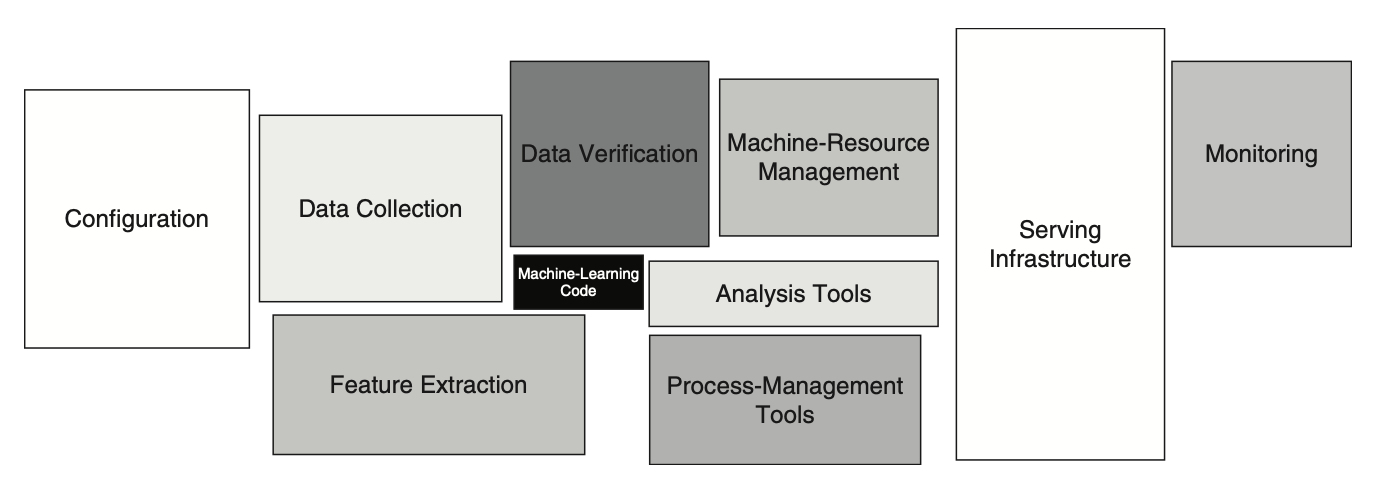
\includegraphics[width=3.5in]{img/x.png}
% \caption{Lines of code, AI-related systems at Google in 2015~\cite{SculleyHGDPECYC15}.
% The tiny black square in the middle is ``core AI'' and the rest are  the standard components of cloud-based S.}\label{google}
% \end{figure}
% Since AI software is software, then the   problems with SE are also problems with AI.
% For example, 
% Conveniently,
% in a ``ship-it'' oriented culture, products are being produced too fast for anyone to
% detect products promoting an unfair advantage.
% With the arrival of generative AI, this trend is  sure to get worse. In the currently AI culture, many products are oriented around large language models that very few people can review, critique or improve. 
Hence I assert that
unfairness is a widespread issue that needs to be addressed and managed. 
Specifically, we need 
to ensure that a software system created by one group, $A$, can be critiqued and modified by another group, $B$.
We say that such a review has several properties:

{\bf It will usually be conducted under some from of time-pressure.}
The kind of 



The more and more time reviewing code (from other sources).
The current evidence is that such reviews often make mistakes,
perhaps since they are often done under some time constraints.

Hence this paper proposes a new benachmark problem: how quickly can we learn ways to change a rpogram's behavior, given li
perhaps due 
Tomorrow's software engineers will spend much time reviewing  model written by someone or something else (e.g. an LLM).  
Given   divergence in   requirements, this review  process  will need 
 to balance   multiple, possibly competing, goals. To be time-effective, these reviews should also  complete without having to label many examples.
 
This task can  characterized  as a   multi-objective  semi-supervised optimization task.   This paper explores
 dozens of such tasks  
The LAB tool
(the Lightweight Adaptive Balancer) 
  was able to use tree-structured Parzen estimators to find large changes that improved
  default behavior  after just seeing 24 labels.
  This result held even when reviewing tens of thousands of examples.  
  
  We hence conclude that tree-structured Parzen estimation
  tools like LAB offer much support for the model  review task. It is especially recommended when there is very little locally labelled data. 
 

 \begin{listing} 
\begin{minted}{python}
class the:  
   # misc settings
   file="data.csv"  # data file
   p=2              # in distance calcs, use a Euclidean distance measure 
   
   # bayes classifier settings
   m=2              #  kludge for hanlding low frequency attribute values
   k=1              #  kludge for handling low frequency classes
   
   # smo settings
   best=0.5         # the n**best labelled items are "best"
   upper=0.8        # after sorting unlabbeled examples, keep top 80%
   label=4          # initially label 4 examples
   Label=16         # label at most another 16 examples

   # sway settings
   Far=0.95         # avoid outliers when seeking distant egs; don't go all the way
   some=256         # only consider some examples when seeking distant examples 
   Min = 0.5        # recursion stops at N^min

   # sway2 settings
   dive=50          # at first, stop at leaves of size 50
   Deeper=4         # next tim around, stop at leaves of size 4
\end{minted}
\caption{{\bf Global settings:} The code uses    control parameters  that referenced in the code using
the idiom (e.g.) ``\texttt{the.file}''.  The semantics of those values are discussed later in this paper.}
\label{listing:the}
\end{listing} 

 
\begin{listing} 
\begin{minted}{python}
class SYM:  # Place to summarize a stream of symbols
  def __init__(self,name=" ",column=0): |\circled{1}|
    self.name, self.column, self.n, self.has = txt, column, 0, Counter() 

  def add(self,x)   : ...   # Add one more count for  symbol `x` |\circled{8}|
  def dist(self,x,y): ...   # Using Aha, return  distance between two syms |\circled{3}|
  def like(self,x,m,prior): # Return likelihood of x is in self  |\circled{4}|
    return (self.has.get(x, 0) + m*prior) / (self.n + m) |\circled{7}|

class NUM: # Place to summarize a stream of numbers
  def __init__(self, name=" ",column=0): |\circled{1}|
   self.name, self.column, self.n = name, at, 0
   self.mu, self.m2, self.sd, self.lo, self.hi  = 0,0,0, 1E30, -1E30
   self.heaven =  0 if txt[-1] == "-" else 1 # if ending with "-", then minimized |\circled{2}| 

  def norm(self,x)   : ... # Return x normalized 0..1, self.lo..self.hi
  def dist(self,x,y) : ... # Using Aha, return distance between two numerics. |\circled{3}|
  def add(self,x)    : ... # Use x to incrementally update lo,hi, mu, and sd |\circled{8}|
  def like(self,x,*_):     # Return prob of x in a normal pdf of self.mu and self.sd |\circled{7}|
    return |$\frac{1}{(\sigma+\epsilon)\sqrt{2\pi}} \exp\left(-(x-\mu)^2/(2\sigma^2 +\epsilon)\right)$| |\circled{6}|
\end{minted}

{\scriptsize 
\circled{1}  NUMs and SYMs   know   column name and  position, plus some other details.\newline 
\circled{2} NUMs  also know their ``heaven'' point; if minimizing, it is 0. Otherwise, it is 1.  \newline
\circled{3} ``\texttt{dist}'' reports the delta between  values using the
Aha et al. formula  from \S\ref{sway}.\newline
\circled{4} ``\texttt{like}'' reports  likelihood that ``x'' belongs to a distribution. \newline
\circled{5}  As per Webb et al.~\cite{yang2002comparative}'s advice,  the $m$ offsets handle low frequencies.   \newline
\circled{6}  $\epsilon=10^{-30}$ added to avoid divide-by-zero issues.\newline 
\circled{7} As per Webb et al.~\cite{yang2002comparative}'s advice,  the $m$ offsets handle low frequencies.   \newline
\circled{8} ``\texttt{add}''   update   distribution. Which for numerics, is via Knuth's method; i.e.\newline
\textcolor{white}{.}\hspace{3mm}$n{\pluseq}1; d=x-\mu; \mu{\pluseq}d/n; \mathit{m2}{\pluseq}d*(x-\mu); \sigma=(m2/(n-1))^{0.5}$} 


\caption{{\bf Column classes}: summarizes  columns into NUMs and SYMs. Some details omitted.} 
\label{listing:numsum}
\end{listing} 
 

 \begin{listing}[!b]
\begin{minted}{python}   
def isNum(s):  return s[0].isupper()  # numerics are upper case  |\two|
def isGoal(s): return s[-1] in "+-"   # goal are to be maximimzed (+) or minimize(-) |\two|  
def isUsed(s): return s[-1] != "X"    # columns ending in "X" are to be ignored. |\two|

class DATA: # Place to hold rows, summarized in the column headers 
  def __init__(self, headerAndRows=[], order=False):
    self.names,*rows = list(headerAndRows)  |\circled{1}|
    self.rows, self.x, self.y = [],[],[] 
    self.cols = [(NUM if isNum(s) else SYM)(s,i) for i,s in enumerate(self.names)]  |\circled{3}|
    [self.add(row) for row in rows]
    if order: self.ordered() |\circled{5}|
    self.also(order)

  def also(self, order=False): |\circled{4}|
    [(self.y if isGoal(c.txt) else self.x).append(col) for c in self.cols if isUsed(c.txt)] 
    
  def add(self,row): # "Add row, summarized in column headers. | \circled{6} |   
    self.rows += [row]
    [col.add(x) for x,col in zip(row,self.cols) if x != "?"] # Avoid 'dont know' values 

  def clone(self, rows=[], order=False): # Return a DATA of same structure with new rows
    return DATA([self.names] + rows, order=order)

  def ordered(self): ...      # Sort rows by distance to heaven 
  def d2h(self,row): ...      # Return Y-distance from row to best Y via Equation |\ref{d2h}|
  def dist(self, row1, row2): # Return X-distance row1 to row2  
    d = sum(c.dist(row1[c.column],row2[c.column])**the.p for c in self.x) |\circled{6} |
    return (d/len(self.x))**(1/the.p)

  def like(self,row,nall,nh,m=1,k=2): # Return log likelihood of row is in self  |\circled{8}| 
    prior = (len(self.rows) + k) / (nall + k*nh)
    tmp   = [col.like(row[col.colulmn], m, prior)  for col in self.x] |\circled{7} |
    return sum(math.log(x) for x in tmp + [prior]) |\circled{9}|
\end{minted}
{\one} Rows arrive as list of lists. Row1 defines column names. Other rows are the examples.\newline
{\two} Column names define the roles of each column.\newline
\circled{3} Columns are stored in \verb+self.cols+.\newline
\circled{4} Further, independent and dependent columns are also store in \verb+self.x,self.y+\newline
\circled{5} Optionally, rows can be sorted by the distance to heaven (Equation~\ref{d2h}).\newline
\circled{6} \RED{dist} is implemented using ``\testtt{dist}'' from Listing~\ref{listing:numsum}.\newline
\circled{7} ``\texttt{like}'' is implemented using ``\testtt{like}'' from Listing~\ref{listing:numsum}.\newline
\circled{8}  As per Webb et al.~\cite{yang2002comparative}'s advice,  the $m,k$ offsets handle low frequencies.   \newline
\circled{9} ``\texttt{like}'' returns log(like) for numerical methods reasons (we can use  small negative numbers rather than very tiny  floats).
\caption{{\bf DATA class} stores rows (and their summaries in column headers). Some details omitted.}
 
\label{listing:1}
\end{listing} 
    
 
LITE and SWAY both use the same underlying object model described in Listing~\ref{listing:1}.   That code uses  the control parameters defined in a class called  \verb+the+ \circled{1} and referenced in the code using
the idiom (e.g.) \verb+the.file+. The semantics of those values are discussed later in this paper.

The code assumes {\eg}s present themselves as a list of lists. The top list 
holds the column names,  which   select the column's role 
Upper case names are numeric columns and everything else is symbolic. \circled{2}.
Names ending in \verb_+-_ are goals to be maximized or minimized. \circled{3}.
The ideal heaven point of a goal being minimized is 0; else it is 1. \circled{4}.


NUM and SYM are classes that summarize columns symbols and numbers respectively.
These classes know their name and column position \circled{5}. 

Lists of NUMs and SYMs are updated by  the DATA class whenever that class
processes a new row \circled{6}

Their summaries are updated by a \verb+add+ method. Thse
\begin{itemize}
    \item x.add(y) 
\end{itemize}code runs over a DATA class that stores rows, 


\begin{listing}[!ht]
\begin{minted}{python}
#class DATA continued
  def smo(self, score=lambda B,R: 2*B-R, fun=None):
    "Predictive modeling to predict if a new example is 'best' or 'rest'"
    def like(row,data):
      "Return log likelihood of row belonging to data"
      return data.like(row, len(data.rows), 2, the.m, the.k)
    def acquire(best, rest, rows):
      "Sort rows best to rest, keep the first (say) 80%"
      chop = int(len(rows) * the.upper)
      return sorted(rows, key=lambda r: -score(like(r,best),like(r,rest)))[:chop]
    #------------------------
    random.shuffle(self.rows)
    done, todo = self.rows[:the.label], self.rows[the.label:]
    data1 = self.clone(done, order=True)
    for i in range(the.Label):
      if len(todo) < 3: break
      n = int(len(done)**the.best + .5)
      top,*todo = acquire(self.clone(data1.rows[:n]),
                          self.clone(data1.rows[n:]),
                          todo)
      done.append(top)
      data1 = self.clone(done, order=True)
    return data1.rows[0],len(data1.rows)
\end{minted}
\caption{Example from the Lua manual}
\label{listing:3}
\end{listing}


\begin{listing}[!ht]
\begin{minted}{python}
#class DATA continued
  def near(self, row1, rows=None): # Return rows, sorted by dist to row1
    return sorted(rows or self.rows, key=lambda row2: self.dist(row1,row2))
    
  def far(self, rows, sortp=False, last=None): # Get 2 distant items, maybe reusing last 
    n     = int(len(rows) * the.Far)
    left  = last or self.near(random.choice(rows),rows)[n]
    right = self.near(left,rows)[n]
    if sortp and self.d2h(right) < self.d2h(left): left,right = right,left
    return left, right

  def half(self, rows, sortp=False, last=None): # divide data by distance to 2 distant egs 
    def dist(r1,r2): return self.dist(r1, r2)
    def proj(row)  : return (dist(row,left)**2 + C**2 - dist(row,right)**2)/(2*C)
    left,right = self.far(random.choices(rows, k=min(the.Half, len(rows))),
                          sortp=sortp, last=last)
    lefts,rights,C = [],[], dist(left,right)
    for n,row in enumerate(sorted(rows, key=proj)):
      (lefts if n < len(rows)/2 else rights).append(row)
    return lefts, rights, left

  def sway(self, rows=None,stop=None,rest=None,evals=1, last=None): # Recurse to best half
    rows = rows or self.rows
    stop = stop or 2*len(rows)**the.Min
    rest = rest or []
    if len(rows) > stop:
      lefts,rights,left  = self.half(rows, True, last)
      return self.sway(lefts, stop, rest+rights, evals+1, left)
    else:
      return rows, rest, evals, last

  def sway3(self): # SWAY twice. Second time, use rows found the first time
    random.shuffle(self.rows);
    rows1, rest1, evals1, __   = self.sway(self.rows, the.dive)
    rows2, rest2, evals2, last = self.sway(rows1, the.Deeper)
    return  rows2, rest1+rest2, evals1 + evals2 + 3, last
\end{minted}
\caption{Example from the Lua manual}
\label{listing:3}
\end{listing}

Supervised learning needs labelled data.
This paper looks for alternatives to supervised learning since,
as listed here,  the SE literature often reports that labelling data is expensive, time-consuming and error-prone.   
\begin{itemize}
\item  
Generating    labels is expensive.
For example, Tu et al.~\cite{tu2020better} cost models report
that it would take   three years relabel the data
from the 714 software projects studied in their  last publication.
\item Not only is labelling expensive, it also is chronically error prone. Numerous labelling errors have been reported in widely used data set for technical debt~\cite{9226105} , security bugs~\cite{ 9371393}; for   static code analysis~\cite{10.1145/3510003.3510214}; or for software code quality~\cite{Shepperd13}.
\item Methods that use no labels ({\em unsupervised learners})
have reported   success in only limited domains such as defect prediction~\cite{XU2021110862};
\item Methods that label just a few examples,  then propagate those values to other examples) have successfully reasoned over 10,000s   records, after labelling just 1 to 2.5\% percent of the data~\cite{10109333,majumder2024less}.
But in those domains, these {\em semi-supervised learners}  still needed
labels for 100s of records.
\item  Human-in-the-loop  {\em active learners}  
minimize human labelling effort by updating their models
each time a human offers an opinion on an example.
Still, even with these tools, the labelling effort can be excessive.
Yu et al.'s active learners need 20\% of the data
labelled, which for (e.g.) 28,750 files in Firefox means labelling 5,750 files ~\cite{yu2019fast2}. Similar values of 10 to 20\% labelling
have been reported by other active learning researchers in SE:
see   Wu et.al~\cite{WU2021106530}.
\item 
Zhang et al.  
Devanbu et al. report that a few dozen full labeled examples (sometimes as few as ten)  are enough for {\em few-shot learning}
to convert large  language models into effective tools
for  
 parsing   test  case output~\cite{le2023log} or translating functions into English~\cite{10.1145/3551349.3559555}. But few-shot learning
 only works where, in the domain being explored, there exists
 a functioning large-language model. As we shall see, there are many domains in SE where this is not true.
\end{itemize}
Another way to look at the labelling problem is not ``how much data do we need'' but ``how fast can we generate high-quality labels?''.  
To explore that question, we first must clarify the phrase ``high-quality label''.

As an example of a ``low-quality labelling scheme'', consider  two graduate students 
 separately skimming over  over  a stream of records,   adding or checking labels.   At the end of the session, the labelling teams meets to discuss and resolve any  disagreements in their labelling. In this way, 100s to 1000s of records can be labelled in a week. Having funded many such sessions\footnote{Using the power of pizza.}, I conjecture that one of the reasons of the above labelling errors is that this approach is so tedious that the labelling team often makes errors.  

 As an example of ``high-quality labelling scheme'', consider labelling exercises run by Richardo Valerdi as he collects data from a panel of subject matter about software cost estimation. One such
 panel is described in 

 

Various semi-supervsed
The point of this apepr is that ll of the above are too much. human time is limited. labelling is epextensive and error prone. predict a change in the maphsis of analutics from model construction to modl reivew.

- very time constrained

- very data constrained

- releatively infrequent (so review session 1 had better produce a moedl taht can be used as a surrogate when the  reviewers are 
unavailable) .

Need a new kind of anaytics, once that is based on very little labels. Based on experience with Promise, can achieve.



Given advances in large language models, 
tomorrow's software engineers will spend much time reviewing  software written by someone or something else (e.g. an LLM).  This review may be part of some legislated  process where a review board of stakeholders (who are unfamiliar with the internals of the software) is  required to decide how best to use some software system.
Given   divergence in stakeholder requirements, this review   will need  to strike a balance between multiple, possibly competing, goals.

XXXXFurther if tomorrow is anything like today, the  review    will be have to be completed quickly before     reviewers are pulled 
aside for  other tasks.

We hece propos that one fugure trend in software analtics,
which is poolry supprot b current methods is model review.

To say that another way, we say that one way to formalize the
model review task  as a  \begin{quote} {\em Multi-objective  semi-supervised optimization task that can access only a  a handful of examples
(say, dozens, not hundreds). }
\end{quote}
This paper asks ``is that task  possible?''. We offer  baseline result
based on a very simple toolkit (less than 400 lines of Pythn). XXXX. We shown that it, yes, indeed it is. 
In dozens of case studies (ranging from
from high-level decisions about software processes to low-level decisions abut how to
configure video encoding software) our LAB tool
(the Lightweight Adaptive Balancer) 
  was able to find large changes that improved
  default behavior of thee systems, after just seeing 24 labels.
  This result held even when reviewing tens of thousands of examples. 
  
  There are three intrestng aspects to this results:
  
- simplicity of the code

- stark contrast to standard practice


- far smaller than prior results
  
  Lest the reader find that result improbable, we offer some a literature review and some maths showing that (a)~there is some precedent in the SE literature for this result, albeit in other domains;
  (b)~there are mathematical reasons to believe that with just  few dozen labels, it is possible to be 95\% confident of finding solutions
  that are statistically indistinguishable from the best solution.  

  
  We hence conclude that tree-structured Parzen estimation
  tools like LAB offer much support for the model  review task. It is especially recommended when there is very little locally labelled data. 

\section{Background}
\subsection{the Problem of Model Review}
The core motivation from this work is to find algorithms that support model review, with very little information.  
 
 
mcintosh2017fix,rahman2013sample,amasaki2020cross

\subsection{Big Data}
  
A commonly expressed belief in machine learning and software analytics
is that the more data, the better.  For example:  
\begin{itemize}
\item
  ``Long-term JIT models should be trained using a cache of
plenty of changes''~\cite{mcintosh2017fix};
\item
  ``..as long as it is large;    (prediction performance) is likely to be boosted more by the sample size''~\cite{rahman2013sample};
  \item
``It is 
natural to think that accumulating multiple releases can be beneficial because
it represents the variability of a project''~\cite{amasaki2020cross}. 
\end{itemize}
Yet sometimes, this ``data-heavy'' approach is not possible. As Devanbu comments: 


\subsection{Few-Short Learning}

\subsection{Active Learning}

Over the years, there have been many results
where   very simple models performed exceptionally well
in both the general AI literature~\cite{Holte1993VerySC,Kohavi97} as
well as in software analytics~\cite{agrawal2019dodge,menzies2008implications}.
Using those results,  it is possible to propose a ``small data''
style of analytics that relies on very simple models.  

\subsection{Why Study Simplifies}
Why is it important to study simple models?  We answer that question in three parts.
Firstly we say that the models generated by sofytwre analytics need to be reviwed.
Secondly, using that cognitive psychologcal theory argues that smaller models are more comprehensible.  
Based on those results, we propose a new style of software analytics
where the goal is to achieve the most, with less resources.  




This paper asks: can do something analogous to  few-shot learning without an a large language model (LLM)?

We explore this since, given advances in large language models, 
tomorrow's software engineers will spend much time reviewing  software written by someone or something else (e.g. an LLM).  This review may be part of some legislated  process where a review board of stakeholders (who are unfamiliar with the internals of the software) is  required to decide how best to use some software system.
Given   divergence in stakeholder requirements, this review   will need  to strike a balance between multiple, possibly competing, goals.
Further if tomorrow is anything like today, the  review    will be have to be completed quickly before     reviewers are pulled 
away for  other tasks. Hence, this review must proceed using only a handful of examples from the local domain.



Some software engineering domains are amenable to big data solutions
where large models are built from vast supplies of background knowledge.
But Devanbu argues that  software engineering,  there are many phenomena that are known to be highly project-specific (e.g. the CPU or time required for one project's usual SQL query may be very different to another).  Such project-specific
data can be quite limited, especially early in the history of a project; thus is it useful to have models 
they can learn to perform a task with very few examples.


When speaking of large language models, Devanbu comments that
a particularly exciting aspect of such learners is their knack for few-shot and zero-shot learning: they can learn to perform a task with very few examples. Few-shoting has particular synergies in software engineering, where there are a lot of phenomena  that are known to be highly project-specific. However, project-specific data can be quite limited, especially early in the history of a project; thus the few-shot learning capacity of such learners might be very relevant.

Here we show that the same effect can be seen in other kinds of learners; specifically, the classifiers used within algorithms called
tree-structured Parzen estimators (TPE) that explore semi-supervised
multi-objective optimization.   TPE is a natural  model for supporting
``time-constrained model-review''; i.e. groups of reviewers who have
 must perpetually review all the different  software systems
 being used in the ever-evolving tool space that surrounds them.
Given recent advances in large language models, and certain changes in the legislative environment around software (see next section),  we antiipate taht such a review proces will become increasingly common 


\section{Features of Time-Constrained Review}

Just to be clear, we are not saying that all problems can be resolved via  few dozen examples. In ultra-safety critical applications, or when building generative models, or (outside of SE) when trying to find another 1\% improvement in (say) the airflow over a wingtip going through the sound barrier, it is required to process as much information as possible.

\subsection{Frequent reviews}

\subsection{Gaps between the reviews}

\section{multi-objective reasonong}

\section{Sem-spervised}

\section{Limited knowledvge of ssytem internals}


Machine learning for busy people should not strive
for (e.g.,) elaborate theories or (e.g.,) increasing the expressive power of the language of the
theory. Rather, a better goal might be to find the smallest theory with the most impact. 

My lesson from working on data sets from the PROMISE conference on rep

\label{intro}
Your text comes here. Separate text sections with
\section{Section title}
\label{sec:1}
Text with citations \cite{RefB} and \cite{RefJ}.
\subsection{Subsection title}
\label{sec:2}
as required. Don't forget to give each section
and subsection a unique label (see Sect.~\ref{sec:1}).
\paragraph{Paragraph headings} Use paragraph headings as needed.
\begin{equation}
a^2+b^2=c^2
\end{equation}

% For one-column wide figures use
\begin{figure}
% Use the relevant command to insert your figure file.
% For example, with the graphicx package use
  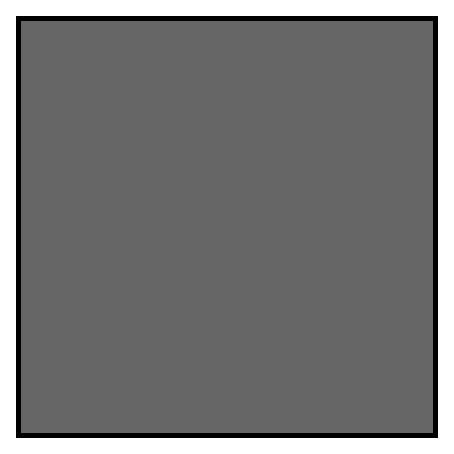
\includegraphics{example.eps}
% figure caption is below the figure
\caption{Please write your figure caption here}
\label{fig:1}       % Give a unique label
\end{figure}
%
% For two-column wide figures use
\begin{figure*}
% Use the relevant command to insert your figure file.
% For example, with the graphicx package use
  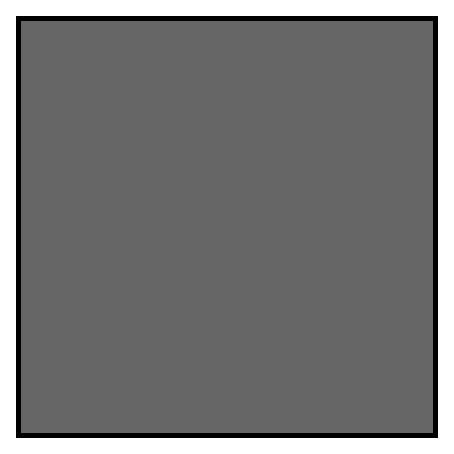
\includegraphics[width=0.75\textwidth]{example.eps}
% figure caption is below the figure
\caption{Please write your figure caption here}
\label{fig:2}       % Give a unique label
\end{figure*}
%
% For tables use
\begin{table}
% table caption is above the table
\caption{Please write your table caption here}
\label{tab:1}       % Give a unique label
% For LaTeX tables use
\begin{tabular}{lll}
\hline\noalign{\smallskip}
first & second & third  \\
\noalign{\smallskip}\hline\noalign{\smallskip}
number & number & number \\
number & number & number \\
\noalign{\smallskip}\hline
\end{tabular}
\end{table}


%\begin{acknowledgements}
%If you'd like to thank anyone, place your comments here
%and remove the percent signs.
%\end{acknowledgements}


% Authors must disclose all relationships or interests that 
% could have direct or potential influence or impart bias on 
% the work: 
%
% \section*{Conflict of interest}
%
% The authors declare that they have no conflict of interest.


% BibTeX users please use one of
%\bibliographystyle{numeric}      % basic style, author-year citations
\bibliographystyle{spmpsci}      % mathematics and physical sciences
%\bibliographystyle{spphys}       % APS-like style for physics
%\bibliography{}   % name your BibTeX data base

% Non-BibTeX users please use
\bibliography{main} 

\end{document}
% end of file template.tex

